

\section*{ID: 88e13c8c}
The total cost $f(x)$, in dollars, to lease a car for 36 months from a particular car dealership is given by $f(x)=36 x+1,000$, where $x$ is the monthly payment, in dollars. What is the total cost to lease a car when the monthly payment is $\$ 400$ ?\\
A. $\$ 13,400$\\
B. $\$ 13,000$\\
C. $\$ 15,400$\\
D. $\$ 37,400$

\section*{ID: 8c5e6702}
A window repair specialist charges $\$ 220$ for the first two hours of repair plus an hourly fee for each additional hour. The total cost for 5 hours of repair is $\$ 400$. Which function $f$ gives the total cost, in dollars, for $x$ hours of repair, where $x \geq 2$ ?\\
A. $f(x)=60 x+100$\\
B. $f(x)=60 x+220$\\
C. $f(x)=80 x$\\
D. $f(x)=80 x+220$

The function $h$ is defined by $h(x)=4 x+28$. The graph of $y=h(x)$ in the $x y$-plane has an $x$-intercept at $(a, 0)$ and a $y$ intercept at $(0, b)$, where $a$ and $b$ are constants. What is the value of $a+b$ ?\\
A. 21\\
B. 28\\
C. 32\\
D. 35

\section*{ID: 2b15d65f}
An economist modeled the demand $Q$ for a certain product as a linear function of the selling price $P$. The demand was 20,000 units when the selling price was \$40 per unit, and the demand was 15,000 units when the selling price was $\$ 60$ per unit. Based on the model, what is the demand, in units, when the selling price is $\$ 55$ per unit?\\
A. 16,250\\
B. 16,500\\
C. 16,750\\
D. 17,500

\section*{ID: be9cb6a2}
The cost of renting a backhoe for up to 10 days is $\$ 270$ for the first day and $\$ 135$ for each additional day. Which of the following equations gives the cost $y$, in dollars, of renting the backhoe for $x$ days, where $x$ is a positive integer and $x \leq 10$ ?\\
A. $y=270 x-135$\\
B. $y=270 x+135$\\
C. $y=135 x+270$\\
D. $y=135 x+135$

\section*{ID: 84664a7c}
The front of a roller-coaster car is at the bottom of a hill and is 15 feet above the ground. If the front of the roller-coaster car rises at a constant rate of 8 feet per second, which of the following equations gives the height $h$, in feet, of the front of the roller-coaster car $s$ seconds after it starts up the hill?\\
A. $h=8 s+15$\\
B. $h=15 s+\frac{335}{8}$\\
c. $h=8 s+\frac{335}{15}$\\
D. $h=15 s+8$

\section*{ID: e62cfe5f}
According to a model, the head width, in millimeters, of a worker bumblebee can be estimated by adding 0.6 to four times the body weight of the bee, in grams. According to the model, what would be the head width, in millimeters, of a worker bumblebee that has a body weight of 0.5 grams?

If $f$ is the function defined by $f(x)=\frac{2 x-1}{3}$, what is the value of $f(5)$ ?\\
A. $\frac{4}{3}$\\
B. $\frac{7}{3}$\\
C. 3\\
D. 9

$$
d=16 t
$$

The given equation represents the distance $d$, in inches, where $t$ represents the number of seconds since an object started moving. Which of the following is the best interpretation of 16 in this context?\\
A. The object moved a total of 16 inches.\\
B. The object moved a total of $16 t$ inches.\\
C. The object is moving at a rate of 16 inches per second.\\
D. The object is moving at a rate of $\frac{1}{16}$ inches per second.

$$
f(x)=39
$$

For the given linear function $f$, which table gives three values of $x$ and their corresponding values of $f(x)$ ?\\
A.

\begin{center}
\begin{tabular}{|c|c|}
\hline
$x$ & $f(x)$ \\
\hline
0 & 0 \\
\hline
1 & 0 \\
\hline
2 & 0 \\
\hline
\end{tabular}
\end{center}

B.

\begin{center}
\begin{tabular}{|c|c|}
\hline
$x$ & $f(x)$ \\
\hline
0 & 39 \\
\hline
1 & 39 \\
\hline
2 & 39 \\
\hline
\end{tabular}
\end{center}

c.

\begin{center}
\begin{tabular}{|c|c|}
\hline
$x$ & $f(x)$ \\
\hline
0 & 0 \\
\hline
1 & 39 \\
\hline
2 & 78 \\
\hline
\end{tabular}
\end{center}

D.

\begin{center}
\begin{tabular}{|c|c|}
\hline
$x$ & $f(x)$ \\
\hline
0 & 39 \\
\hline
1 & 0 \\
\hline
2 & -39 \\
\hline
\end{tabular}
\end{center}












\section*{ID: e470e19d}
The function $f$ is defined by $f(x)=7 x-84$. What is the $x$-intercept of the graph of $y=f(x)$ in the $x y$-plane?\\
A. $(-12,0)$\\
B. $(-7,0)$\\
C. $(7,0)$\\
D. $(12,0)$

\begin{center}
\begin{tabular}{|c|c|c|c|c|}
\hline
$x$ & 10 & 15 & 20 & 25 \\
\hline
$f(x)$ & 82 & 137 & 192 & 247 \\
\hline
\end{tabular}
\end{center}

The table shows four values of $x$ and their corresponding values of $f(x)$. There is a linear relationship between $x$ and $f(x)$ that is defined by the equation $f(x)=m x-28$, where $m$ is a constant. What is the value of $m$ ?\\
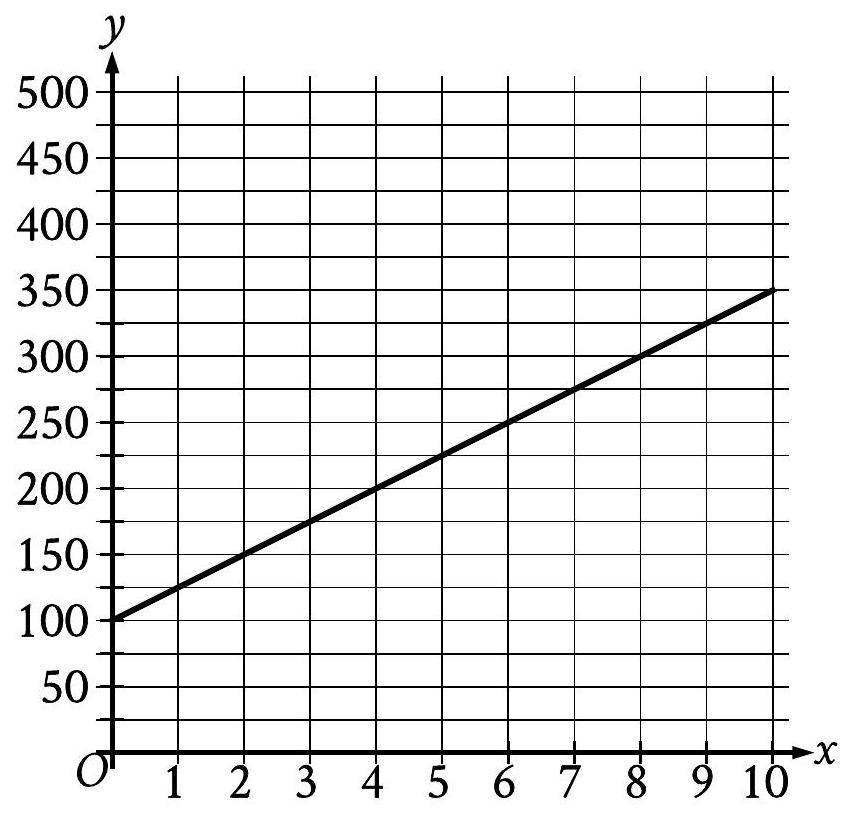
\includegraphics[max width=\textwidth, center]{2025_06_15_1eff2981bb1cf12f04f1g-23}

The graph of the function $f$, where $y=f(x)$, gives the total cost $y$, in dollars, for a certain video game system and $x$ games. What is the best interpretation of the slope of the graph in this context?\\
A. Each game costs $\$ 25$.\\
B. The video game system costs $\$ 100$.\\
C. The video game system costs $\$ 25$.\\
D. Each game costs $\$ 100$.

\section*{ID: b988eeec}
The functions $f$ and $g$ are defined as $f(x)=\frac{1}{4} x-9$ and $g(x)=\frac{3}{4} x+21$. If the function $h$ is defined as $h(x)=f(x)+g(x)$, what is the $x$-coordinate of the $x$-intercept of the graph of $y=h(x)$ in the $x y$-plane?

\section*{ID: 13294295}
The graph shown models the number of candy bars a certain machine wraps with a label in $x$ seconds.\\
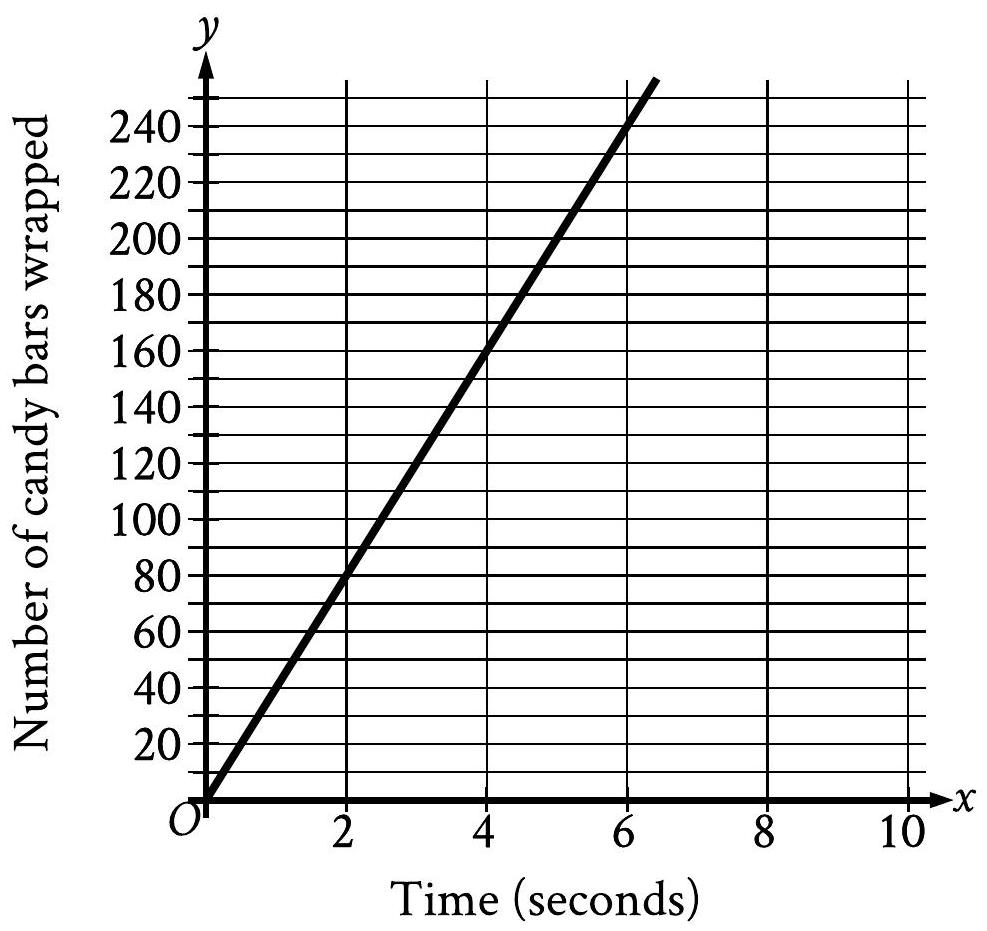
\includegraphics[max width=\textwidth, center]{2025_06_15_1eff2981bb1cf12f04f1g-25}

According to the graph, what is the estimated number of candy bars the machine wraps with a label per second?\\
A. 2\\
B. 40\\
C. 78\\
D. 80

\section*{ID: 3e9eaffc}
Caleb used juice to make popsicles. The function $f(x)=-5 x+30$ approximates the volume, in fluid ounces, of juice Caleb had remaining after making $x$ popsicles. Which statement is the best interpretation of the $y$-intercept of the graph of $y=f(x)$ in the $x y$-plane in this context?\\
A. Caleb used approximately 5 fluid ounces of juice for each popsicle.\\
B. Caleb had approximately 5 fluid ounces of juice when he began to make the popsicles.\\
C. Caleb had approximately 30 fluid ounces of juice when he began to make the popsicles.\\
D. Caleb used approximately 30 fluid ounces of juice for each popsicle.

\section*{ID: af2ba762}
According to data provided by the US Department of Energy, the average price per gallon of regular gasoline in the United States from September 1, 2014, to December 1, 2014, is modeled by the function $F$ defined below, where $F(x)$ is the average price per gallon $x$ months after September 1 .\\
$F(x)=2.74-0.19(x-3)$

The constant 2.74 in this function estimates which of the following?\\
A. The average monthly decrease in the price per gallon\\
B. The difference in the average price per gallon from September 1, 2014, to December 1, 2014\\
C. The average price per gallon on September 1, 2014\\
D. The average price per gallon on December 1, 2014

\section*{ID: a775af14}
In the $x y$-plane, the graph of the linear function $f$ contains the points $(0,2)$ and $(8,34)$. Which equation defines $f$, where $y=f(x)$ ?\\
A. $f(x)=2 x+42$\\
B. $f(x)=32 x+36$\\
C. $f(x)=4 x+2$\\
D. $f(x)=8 x+2$

\section*{ID: b8cbe394}
Sean rents a tent at a cost of $\$ 11$ per day plus a onetime insurance fee of $\$ 10$. Which equation represents the total cost $c$, in dollars, to rent the tent with insurance for $d$ days?\\
A. $c=11(d+10)$\\
B. $c=10(d+11)$\\
C. $c=11 d+10$\\
D. $c=10 d+11$

\section*{ID: dae126d7}
The boiling point of water at sea level is 212 degrees Fahrenheit $\left({ }^{\circ} \mathrm{F}\right)$. For every 550 feet above sea level, the boiling point of water is lowered by about $1^{\circ} \mathrm{F}$. Which of the following equations can be used to find the boiling point $B$ of water, in ${ }^{\circ} \mathrm{F}, x$ feet above sea level?\\
A. $B=550+\frac{x}{212}$\\
B. $B=550-\frac{x}{212}$\\
C. $B=212+\frac{x}{550}$\\
D. $B=212-\frac{x}{550}$

\begin{center}
\begin{tabular}{|c|c|}
\hline
$x$ & $f(x)$ \\
\hline
1 & 5 \\
\hline
3 & 13 \\
\hline
5 & 21 \\
\hline
\end{tabular}
\end{center}

Some values of the linear function $f$ are shown in the table above. Which of the following defines $f$ ?\\
A. $f(x)=2 x+3$\\
B. $f(x)=3 x+2$\\
C. $f(x)=4 x+1$\\
D. $f(x)=5 x$

\section*{ID: 70d9516e}
A bus is traveling at a constant speed along a straight portion of road. The equation $d=30 t$ gives the distance $d$, in feet from a road marker, that the bus will be $t$ seconds after passing the marker. How many feet from the marker will the bus be 2 seconds after passing the marker?\\
A. 30\\
B. 32\\
C. 60\\
D. 90

The cost $y$, in dollars, for a manufacturer to make $x$ rings is represented by the line shown.\\
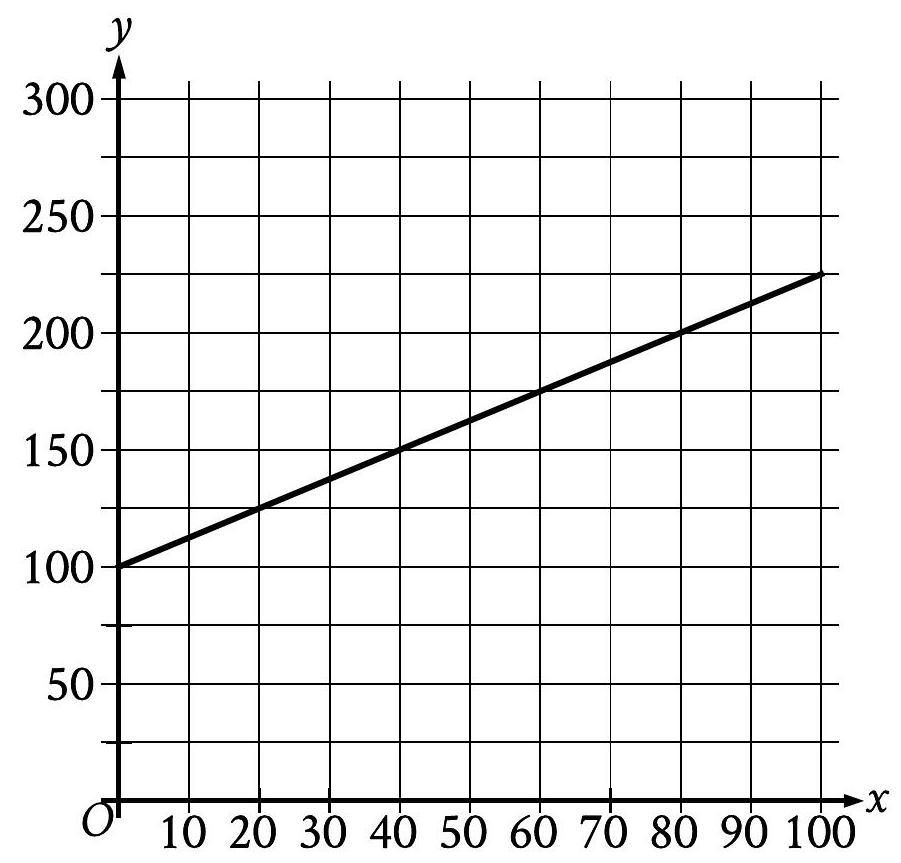
\includegraphics[max width=\textwidth, center]{2025_06_15_1eff2981bb1cf12f04f1g-33}

What is the cost, in dollars, for the manufacturer to make 60 rings?\\
A. 100\\
B. 125\\
C. 175\\
D. 225

\section*{ID: 271f7e3f}
$$
f(x)=\frac{(x+7)}{4}
$$

For the function $f$ defined above, what is the value of $f(9)-f(1)$ ?\\
A. 1\\
B. 2\\
C. $\frac{1}{4}$\\
D. $\frac{9}{4}$

\section*{ID: f79fffba}
The function $h$ is defined by $h(x)=3 x-7$. What is the value of $h(-2)$ ?\\
A. -13\\
B. -10\\
C. 10\\
D. 13

\section*{ID: a9039591}
\begin{center}
\begin{tabular}{|c|c|}
\hline
$x$ & $f(x)$ \\
\hline
0 & 29 \\
\hline
1 & 32 \\
\hline
2 & 35 \\
\hline
\end{tabular}
\end{center}

For the linear function $f$, the table shows three values of $x$ and their corresponding values of $f(x)$. Which equation defines $f(x)$ ?\\
A. $f(x)=3 x+29$\\
B. $f(x)=29 x+32$\\
C. $f(x)=35 x+29$\\
D. $f(x)=32 x+35$

\section*{ID: a396ed75}
For a training program, Juan rides his bike at an average rate of 5.7 minutes per mile. Which function $m$ models the number of minutes it will take Juan to ride $x$ miles at this rate?\\
A. $m(x)=\frac{x}{5.7}$\\
B. $m(x)=x+5.7$\\
C. $m(x)=x-5.7$\\
D. $m(x)=5.7 x$

\section*{ID: 50f4cb9c}
\begin{center}
\begin{tabular}{|c|c|}
\hline
$x$ & $f(x)$ \\
\hline
1 & -64 \\
\hline
2 & 0 \\
\hline
3 & 64 \\
\hline
\end{tabular}
\end{center}

For the linear function $f$, the table shows three values of $x$ and their corresponding values of $f(x)$. Function $f$ is defined by $f(x)=a x+b$, where $a$ and $b$ are constants. What is the value of $a-b$ ?\\
A. -64\\
B. 62\\
C. 128\\
D. 192

\section*{ID: 16889ef3}
Oil and gas production in a certain area dropped from 4 million barrels in 2000 to 1.9 million barrels in 2013. Assuming that the oil and gas production decreased at a constant rate, which of the following linear functions $f$ best models the production, in millions of barrels, $t$ years after the year 2000?\\
A. $f(t)=\frac{21}{130} t+4$\\
B. $f(t)=\frac{19}{130} t+4$\\
C. $f(t)=-\frac{21}{130} t+4$\\
D. $f(t)=-\frac{19}{130} t+4$

ID: c651cc56

\begin{center}
\begin{tabular}{|c|c|}
\hline
$x$ & $f(x)$ \\
\hline
0 & -2 \\
\hline
2 & 4 \\
\hline
6 & 16 \\
\hline
\end{tabular}
\end{center}

Some values of the linear function $f$ are shown in the table above. What is the value of $f(3)$ ?\\
A. 6\\
B. 7\\
C. 8\\
D. 9

In the $x y$-plane, the points $(-2,3)$ and $(4,-5)$ lie on the graph of which of the following linear functions?\\
A. $f(x)=x+5$\\
B. $f(x)=\frac{1}{2} x+4$\\
c. $f(x)=-\frac{4}{3} x+\frac{1}{3}$\\
D. $f(x)=-\frac{3}{2} x+1$

\section*{ID: 11e1ab81}
\begin{center}
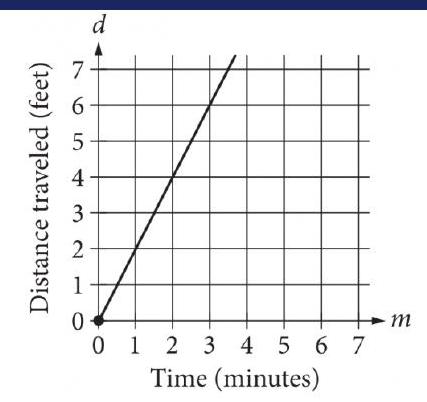
\includegraphics[max width=\textwidth]{2025_06_15_1eff2981bb1cf12f04f1g-42}
\end{center}

The graph above shows the distance traveled $d$, in feet, by a product on a conveyor belt $m$ minutes after the product is placed on the belt. Which of the following equations correctly relates $d$ and $m$ ?\\
A. $d=2 m$\\
B. $d=\frac{1}{2} m$\\
C. $d=m+2$\\
D. $d=2 m+2$

$$
c(x)=m x+500
$$

A company's total cost $c(x)$, in dollars, to produce $x$ shirts is given by the function above, where $m$ is a constant and $\boldsymbol{x}>0$. The total cost to produce 100 shirts is \$800. What is the total cost, in dollars, to produce 1000 shirts? (Disregard the \$ sign when gridding your answer.)

\section*{ID: a309803e}
One gallon of paint will cover 220 square feet of a surface. A room has a total wall area of $w$ square feet. Which equation represents the total amount of paint $P$, in gallons, needed to paint the walls of the room twice?\\
A. $P=\frac{w}{110}$\\
B. $P=440 w$\\
C. $P=\frac{w}{220}$\\
D. $P=220 w$

\section*{ID: bf883fde}
For the function $f$, the graph of $y=f(x)$ in the $x y$-plane has a slope of 3 and passes through the point $(0,-8)$. Which equation defines $f$ ?\\
A. $f(x)=3 x$\\
B. $f(x)=3 x-8$\\
C. $f(x)=3 x+5$\\
D. $f(x)=3 x+11$

\section*{ID: 3462d850}
Marisol drove 3 hours from City A to City B. The equation below estimates the distance $d$, in miles, Marisol traveled after driving for $t$ hours.\\
$d=45 t$

Which of the following does 45 represent in the equation?\\
A. Marisol took 45 trips from City A to City B.\\
B. The distance between City A and City B is 45 miles.\\
C. Marisol drove at an average speed of about 45 miles per hour.\\
D. It took Marisol 45 hours to drive from City A to City B.

A linear model estimates the population of a city from 1991 to 2015. The model estimates the population was 57 thousand in 1991,224 thousand in 2011 , and $x$ thousand in 2015 . To the nearest whole number, what is the value of $x$ ?

\section*{ID: 23dedddd}
In the linear function $f, f(0)=8$ and $f(1)=12$. Which equation defines $f$ ?\\
A. $f(x)=12 x+8$\\
B. $f(x)=4 x$\\
C. $f(x)=4 x+12$\\
D. $f(x)=4 x+8$

$$
f(x)=2 x+244
$$

The given function $f$ represents the perimeter, in centimeters (cm), of a rectangle with a length of $x \mathrm{~cm}$ and a fixed width. What is the width, in cm , of the rectangle?\\
A. 2\\
B. 122\\
C. 244\\
D. 488

$$
w(t)=300-4 t
$$

The function $w$ models the volume of liquid, in milliliters, in a container $t$ seconds after it begins draining from a hole at the bottom. According to the model, what is the predicted volume, in milliliters, draining from the container each second?\\
A. 300\\
B. 296\\
C. 75\\
D. 4

$$
F(x)=\frac{9}{5}(x-273.15)+32
$$

The function $F$ gives the temperature, in degrees Fahrenheit, that corresponds to a temperature of $x$ kelvins. If a temperature increased by 2.10 kelvins, by how much did the temperature increase, in degrees Fahrenheit?\\
A. 3.78\\
B. 35.78\\
C. 487.89\\
D. 519.89

$$
s=40+3 t
$$

The equation gives the speed $s$, in miles per hour, of a certain car $t$ seconds after it began to accelerate. What is the speed, in miles per hour, of the car 5 seconds after it began to accelerate?\\
A. 40\\
B. 43\\
C. 45\\
D. 55

$$
T=1,000+18 h
$$

In the equation above, $T$ represents Brittany's total take-home pay, in dollars, for her first week of work, where $h$ represents the number of hours she worked that week and 1,000 represents a sign-on bonus. If Brittany's total take-home pay was $\$ 1,576$, for how many hours was Brittany paid for her first week of work?\\
A. 16\\
B. 32\\
C. 55\\
D. 88

\section*{ID: a1696f3e}
The function $g$ is defined as $g(x)=5 x+a$, where $a$ is a constant. If $g(4)=31$, what is the value of $a$ ?\\
A. 30\\
B. 22\\
C. 11\\
D. -23

$$
j(x)=m x+144
$$

For the linear function $j, m$ is a constant and $j(12)=18$. What is the value of $j(10)$ ?

\section*{ID: 868fc236}
Energy per Gram of Typical Macronutrients

\begin{center}
\begin{tabular}{|l|c|c|}
\hline
Macronutrient & Food calories & Kilojoules \\
\hline
Protein & 4.0 & 16.7 \\
\hline
Fat & 9.0 & 37.7 \\
\hline
Carbohydrate & 4.0 & 16.7 \\
\hline
\end{tabular}
\end{center}

The table above gives the typical amounts of energy per gram, expressed in both food calories and kilojoules, of the three macronutrients in food. If $x$ food calories is equivalent to $k$ kilojoules, of the following, which best represents the relationship between $x$ and $k$ ?\\
A. $k=0.24 x$\\
B. $k=4.2 x$\\
C. $x=4.2 \mathrm{k}$\\
D. $x k=4.2$

\section*{ID: 7e1bff94}
The table gives the number of hours, $h$, of labor and a plumber's total charge $f(h)$, in dollars, for two different jobs.

\begin{center}
\begin{tabular}{|c|c|}
\hline
$h$ & $f(h)$ \\
\hline
1 & 155 \\
\hline
3 & 285 \\
\hline
\end{tabular}
\end{center}

There is a linear relationship between $h$ and $f(h)$. Which equation represents this relationship?\\
A. $f(h)=25 h+130$\\
B. $f(h)=130 h+25$\\
C. $f(h)=65 h+90$\\
D. $f(h)=90 h+65$

\section*{ID: Ocadb20e}
The function $f$ is defined by $f(x)=\frac{x+15}{5}$, and $f(a)=10$, where $a$ is a constant. What is the value of $a$ ?\\
A. 5\\
B. 10\\
C. 35\\
D. 65

The function $f$ is defined by the equation $f(x)=100 x+2$. What is the value of $f(x)$ when $x=9$ ?\\
A. 111\\
B. 118\\
C. 900\\
D. 902

\section*{ID: 042aa429}
If $f(x)=x+7$ and $g(x)=7 x$, what is the value of $4 f(2)-g(2)$ ?\\
A. -5\\
B. 1\\
C. 22\\
D. 28

\section*{ID: de6fe450}
On January 1, 2015, a city's minimum hourly wage was $\$ 9.25$. It will increase by $\$ 0.50$ on the first day of the year for the next 5 years. Which of the following functions best models the minimum hourly wage, in dollars, $x$ years after January 1, 2015, where $x=1,2,3,4,5$ ?\\
A. $f(x)=9.25-0.50 x$\\
B. $f(x)=9.25 x-0.50$\\
C. $f(x)=9.25+0.50 x$\\
D. $f(x)=9.25 x+0.50$

\section*{ID: cee5b352}
The length, $y$, of a white whale was 162 centimeters (cm) when it was born and increased an average of 4.8 cm per month for the first 12 months after it was born. Which equation best represents this situation, where $x$ is the number of months after the whale was born and $y$ is the length, in cm , of the whale?\\
A. $y=162 x$\\
B. $y=162 x+162$\\
C. $y=4.8 x+4.8$\\
D. $y=4.8 x+162$

ID: 78391 fcc

\begin{center}
\begin{tabular}{|c|c|c|c|c|}
\hline
$x$ & -11 & -10 & -9 & -8 \\
\hline
$f(x)$ & 21 & 18 & 15 & 12 \\
\hline
\end{tabular}
\end{center}

The table above shows some values of $x$ and their corresponding values $f(x)$ for the linear function $f$. What is the $x$-intercept of the graph of $y=f(x)$ in the $x y$ plane?\\
A. $(-3,0)$\\
B. $(-4,0)$\\
C. $(-9,0)$\\
D. $(-12,0)$

\section*{ID: aad7e1b9}
The function $f$ is defined by $f(x)=\frac{1}{10} x-2$. What is the $y$-intercept of the graph of $y=f(x)$ in the $x y$-plane?\\
A. $(-2,0)$\\
B. $(0,-2)$\\
C. $\left(0, \frac{1}{10}\right)$\\
D. $\left(\frac{1}{10}, 0\right)$

\section*{ID: 1bc11c4e}
$$
g(m)=-0.05 m+12.1
$$

The given function $g$ models the number of gallons of gasoline that remains from a full gas tank in a car after driving $m$ miles. According to the model, about how many gallons of gasoline are used to drive each mile?\\
A. 0.05\\
B. 12.1\\
C. 20\\
D. 242.0

The equation above represents the speed $y$, in feet per second, of Sheila's bicycle $x$ seconds after she applied the brakes at the end of a ride. If the equation is graphed in the $x y$-plane, which of the following is the best interpretation of the $x$-coordinate of the line's $x$-intercept in the context of the problem?\\
A. The speed of Sheila's bicycle, in feet per second, before Sheila applied the brakes\\
B. The number of feet per second the speed of Sheila's bicycle decreased each second after Sheila applied the brakes\\
C. The number of seconds it took from the time Sheila began applying the brakes until the bicycle came to a complete stop\\
D. The number of feet Sheila's bicycle traveled from the time she began applying the brakes until the bicycle came to a complete stop

\section*{ID: 6efcc0a3}
In the linear function $h, h(0)=41$ and $h(1)=40$. Which equation defines $h$ ?\\
A. $h(x)=-x+41$\\
B. $h(x)=-x$\\
C. $h(x)=-41 x$\\
D. $h(x)=-41$

\section*{ID: 776cfa7c}
Hana deposited a fixed amount into her bank account each month. The function $f(t)=100+25 t$ gives the amount, in dollars, in Hana's bank account after $t$ monthly deposits. What is the best interpretation of 25 in this context?\\
A. With each monthly deposit, the amount in Hana's bank account increased by $\$ 25$.\\
B. Before Hana made any monthly deposits, the amount in her bank account was $\$ 25$.\\
C. After 1 monthly deposit, the amount in Hana's bank account was $\$ 25$.\\
D. Hana made a total of 25 monthly deposits.

The function $f$ is defined by $f(x)=5 x+8$. For what value of $x$ does $f(x)=58$ ?\\
A. 10\\
B. 13\\
C. 50\\
D. 298

The function $h$ is defined by $h(x)=x+200$. What is the value of $h(50)$ ?\\
A. 200\\
B. 250\\
C. 10,000\\
D. 50,200

Energy per Gram of Typical Macronutrients

\begin{center}
\begin{tabular}{|l|c|c|}
\hline
Macronutrient & Food calories & Kilojoules \\
\hline
Protein & 4.0 & 16.7 \\
\hline
Fat & 9.0 & 37.7 \\
\hline
Carbohydrate & 4.0 & 16.7 \\
\hline
\end{tabular}
\end{center}

The table above gives the typical amounts of energy per gram, expressed in both food calories and kilojoules, of the three macronutrients in food. If the 180 food calories in a granola bar come entirely from $p$ grams of protein, $f$ grams of fat, and $c$ grams of carbohydrate, which of the following expresses $f$ in terms of $p$ and $c$ ?\\
A. $f=20+\frac{4}{9}(p+c)$\\
B. $f=20-\frac{4}{9}(p+c)$\\
c. $f=20-\frac{4}{9}(p-c)$\\
D. $f=20+\frac{9}{4}(p+c)$

\section*{ID: daad7c32}
An object hangs from a spring. The formula $\ell=30+2 w$ relates the length $\ell$, in centimeters, of the spring to the weight $w$, in newtons, of the object. Which of the following describes the meaning of the 2 in this context?\\
A. The length, in centimeters, of the spring with no weight attached\\
B. The weight, in newtons, of an object that will stretch the spring 30 centimeters\\
C. The increase in the weight, in newtons, of the object for each one-centimeter increase in the length of the spring\\
D. The increase in the length, in centimeters, of the spring for each one-newton increase in the weight of the object

For the function $f$, if $f(3 x)=x-6$ for all values of $x$, what is the value of $f(6)$ ?\\
A. -6\\
B. -4\\
C. 0\\
D. 2

\section*{ID: 441558e7}
Scientists collected fallen acorns that each housed a colony of the ant species P. ohioensis and analyzed each colony's structure. For any of these colonies, if the colony has $x$ worker ants, the equation $y=0.67 x+2.6$ where $20 \leq x \leq 110$, gives the predicted number of larvae, $y$, in the colony. If one of these colonies has 58 worker ants, which of the following is closest to the predicted number of larvae in the colony?\\
A. 41\\
B. 61\\
C. 83\\
D. 190

The graph of the function $f$ is a line in the $x y$-plane. If the line has slope $\frac{3}{4}$ and $f(0)=3$, which of the following defines $f$ ?\\
A. $f(x)=\frac{3}{4} x-3$\\
B. $f(x)=\frac{3}{4} x+3$\\
C. $f(x)=4 x-3$\\
D. $f(x)=4 x+3$\\
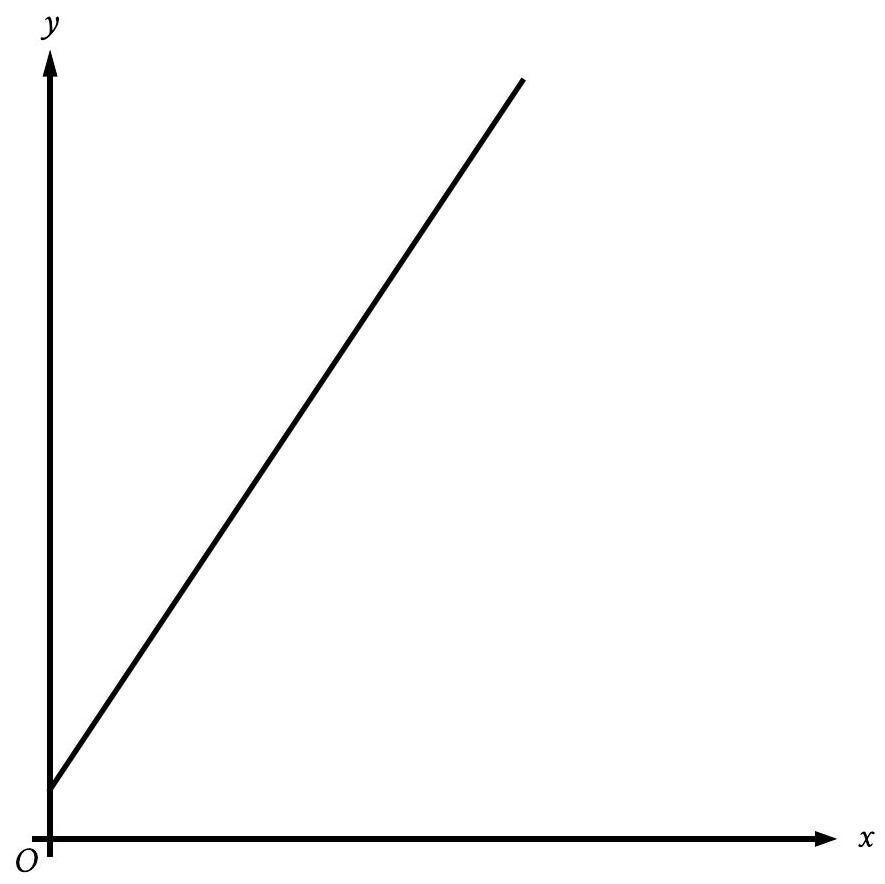
\includegraphics[max width=\textwidth, center]{2025_06_15_1eff2981bb1cf12f04f1g-76}

The graph represents the total charge, in dollars, by an electrician for $x$ hours of work. The electrician charges a onetime fee plus an hourly rate. What is the best interpretation of the slope of the graph?\\
A. The electrician's hourly rate\\
B. The electrician's onetime fee\\
C. The maximum amount that the electrician charges\\
D. The total amount that the electrician charges

\section*{ID: 0ea7ef01}
Oxygen gas is placed inside a tank with a constant volume. The graph shows the estimated temperature $y$, in kelvins, of the oxygen gas when its pressure is $x$ atmospheres.\\
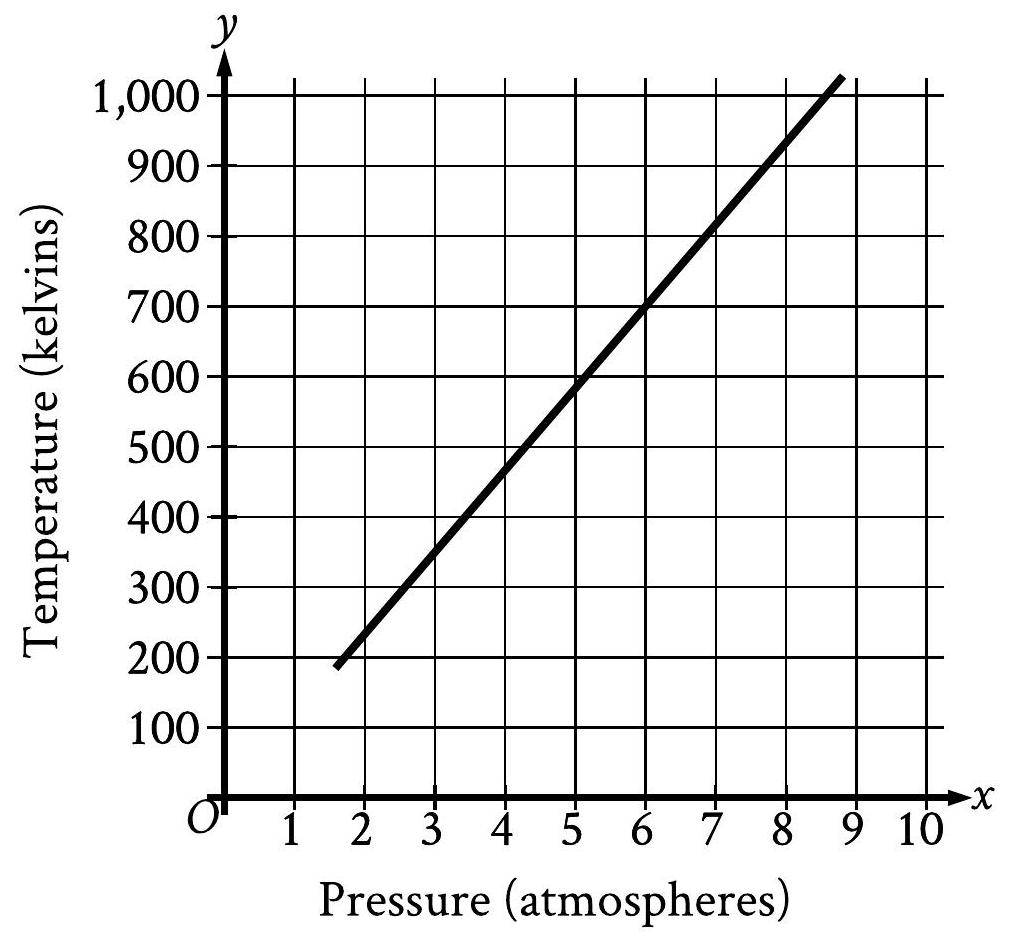
\includegraphics[max width=\textwidth, center]{2025_06_15_1eff2981bb1cf12f04f1g-77}

What is the estimated temperature, in kelvins, of the oxygen gas when its pressure is 6 atmospheres?\\
A. 6\\
B. 60\\
C. 700\\
D. 760

\section*{ID: 1ecaa9c0}
Robert rented a truck to transport materials he purchased from a hardware store. He was charged an initial fee of $\$ 20.00$ plus an additional $\$ 0.70$ per mile driven. If the truck was driven 38 miles, what was the total amount Robert was charged?\\
A. $\$ 46.60$\\
B. $\$ 52.90$\\
C. $\$ 66.90$\\
D. $\$ 86.50$

$$
f(x)=2 x+3
$$

For the given function $f$, the graph of $y=f(x)$ in the $x y$-plane is parallel to line $j$. What is the slope of line $j$ ?

The function $f$ is defined by $f(x)=m x+b$, where $m$ and $b$ are constants. If $f(0)=18$ and $f(1)=20$, what is the value of $m$ ?

\section*{ID: 8643d906}
$P(t)=250+10 t$

The population of snow leopards in a certain area can be modeled by the function $P$ defined above, where $P(t)$ is the population $t$ years after 1990. Of the following, which is the best interpretation of the equation $P(30)=550$ ?\\
A. The snow leopard population in this area is predicted to be 30 in the year 2020.\\
B. The snow leopard population in this area is predicted to be 30 in the year 2030.\\
C. The snow leopard population in this area is predicted to be 550 in the year 2020.\\
D. The snow leopard population in this area is predicted to be 550 in the year 2030.

\section*{ID: bbf9e5ce}
For groups of 25 or more people, a museum charges $\$ 21$ per person for the first 25 people and $\$ 14$ for each additional person. Which function $f$ gives the total charge, in dollars, for a tour group with $n$ people, where $n \geq 25$ ?\\
A. $f(n)=14 n+175$\\
B. $f(n)=14 n+525$\\
C. $f(n)=35 n-350$\\
D. $f(n)=14 n+21$

If $y=5 x+10$, what is the value of $y$ when $x=8$ ?

\section*{ID: 41fdc0b8}
Population of Greenleaf, Idaho

\begin{center}
\begin{tabular}{|c|c|}
\hline
Year & Population \\
\hline
2000 & 862 \\
\hline
2010 & 846 \\
\hline
\end{tabular}
\end{center}

The table above shows the population of Greenleaf, Idaho, for the years 2000 and 2010. If the relationship between population and year is linear, which of the following functions $P$ models the population of Greenleaf $t$ years after 2000?\\
A. $P(t)=862-1.6 t$\\
B. $P(t)=862-16 t$\\
c. $P(t)=862+16(t-2,000)$\\
D. $P(t)=862-1.6(t-2,000)$

\section*{ID: a73a5c22}
The function $g$ is defined by $g(x)=10 x+8$. What is the value of $g(x)$ when $x=8$ ?\\
A. 0\\
B. 8\\
C. 10\\
D. 88

$$
f(x)=7 x+1
$$

The function gives the total number of people on a company retreat with $x$ managers. What is the total number of people on a company retreat with 7 managers?

Which of the following is the graph of the equation $y=2 x-5$ in the $x y$-plane?\\
A.\\
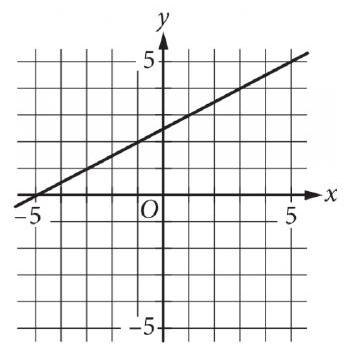
\includegraphics[max width=\textwidth, center]{2025_06_15_1eff2981bb1cf12f04f1g-87}\\
B.\\
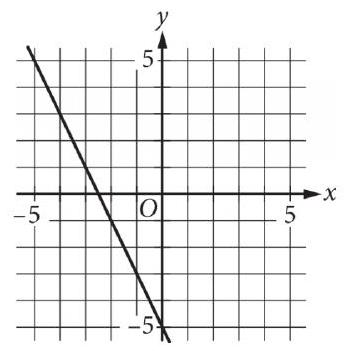
\includegraphics[max width=\textwidth, center]{2025_06_15_1eff2981bb1cf12f04f1g-87(3)}\\
C.\\
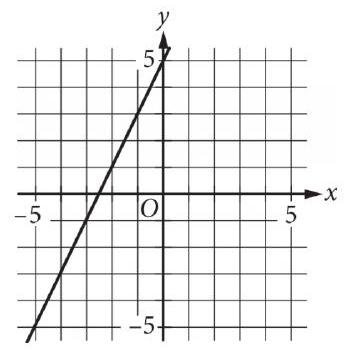
\includegraphics[max width=\textwidth, center]{2025_06_15_1eff2981bb1cf12f04f1g-87(2)}\\
D.\\
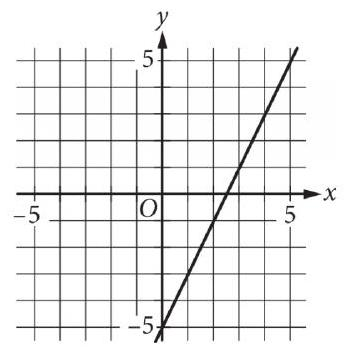
\includegraphics[max width=\textwidth, center]{2025_06_15_1eff2981bb1cf12f04f1g-87(1)}


